\section{Spektren}
\subsection{Kosinus- und Sinus-Amplitude Diagramm}
Abtragen der $a_n$ und $b_n$ zu den entsprechenden $\omega$ Werten:\\
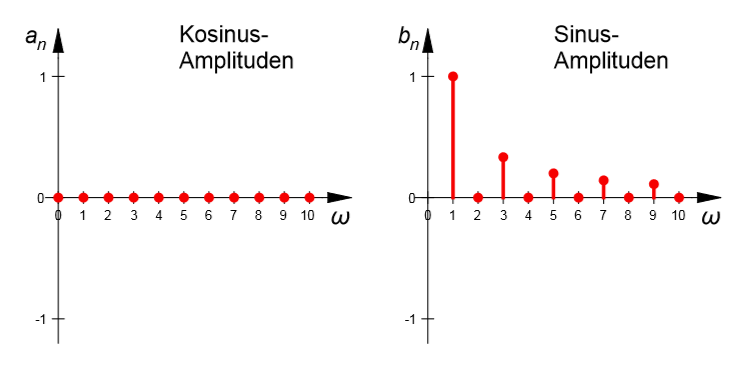
\includegraphics[width=\columnwidth]{Images/amplituden_diagram}


\subsection{Amplituden-/Phasendiagramm $\mathbb{R}$}
Fasst die Koeffizienten zur Komplexen Amplitude und Phasenverschiebung zusammen.\\
\[
A_n = \left|a_n - jb_n\right| = \sqrt{a_n^2 + b_n^2} \qquad \varphi_n = \arg(a_n - jb_n)
\]
Wobei für $A_0 = \frac{a_0}{2}$ und $\varphi_0 = \arg(a_0)$ gilt.

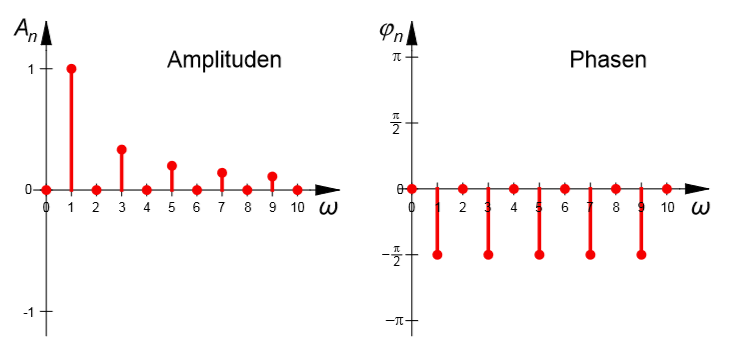
\includegraphics[width=\columnwidth]{Images/phasen_diagram}

\noindent\textbf{Tip:} Siehe auch \ref{umrechnung} für die $\mathbb{C}$ Darstellung.

\subsection{Amplituden-/Phasendiagramm $\mathbb{C}$}
Gleich wie $\mathbb{R}$ Diagramm, nur werden die entsprechenden $c_n$ abgetragen.\\
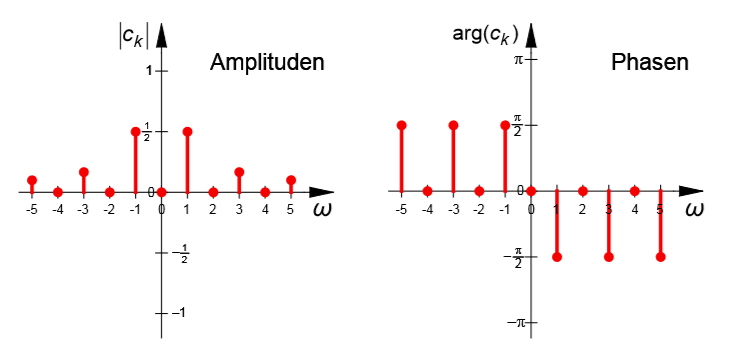
\includegraphics[width=\columnwidth]{Images/phasen_diagram_complex}

\noindent\textbf{Tip:} Die Achsensymmetrie im Amplituden- und Punktsymmetrie im Phasen-Diagramm sind für alle Funktionen gegeben. Siehe auch \ref{umrechnung} für die $\mathbb{R}$ Darstellung.